%!TEX root = da2020-03.tex

\Chapter{3}{\tPN{}~Model: Port~Numbering}

\noindent
Now that we have introduced the essential graph-theoretic concepts, we are ready to define what a ``distributed algorithm'' is. In this chapter, we will study one variant of the theme: deterministic distributed algorithms in the ``port-numbering model''. We will use the abbreviation $\PN$ for the port-numbering model, and we will also use the term ``$\PN$-algorithm'' to refer to deterministic distributed algorithms in the port-numbering model. For now, everything will be deterministic\mydash randomized algorithms will be discussed in later chapters.

\section{Introduction}

The basic idea of the $\PN$ model is best explained through an example. Suppose that I claim the following:
\begin{itemize}
    \item $A$ is a deterministic distributed algorithm that finds a \Apx{2} of a minimum vertex cover in the port-numbering model.
\end{itemize}
Or, in brief:
\begin{itemize}
    \item $A$ is a $\PN$-algorithm for finding a \Apx{2} of a minimum vertex cover.
\end{itemize}
Informally, this entails the following:
\begin{enumerate}
    \item We can take any simple undirected graph $G = (V,E)$.
    \item We can then put together a computer network $N$ with the same structure as $G$. A node $v \in V$ corresponds to a computer in $N$, and an edge $\{u,v\} \in E$ corresponds to a communication link between the computers $u$ and $v$.
    \item Communication takes place through communication ports. A node of degree $d$ corresponds to a computer with $d$ ports that are labeled with numbers $1, 2, \dotsc, d$ in an arbitrary order.
    \item Each computer runs a copy of the same deterministic algorithm $A$. All nodes are identical; initially they know only their own degree (i.e., the number of communication ports).
    \item All computers are started simultaneously, and they follow algorithm $A$ synchronously in parallel. In each synchronous communication round, all computers in parallel
    \begin{enumerate}[label=(\arabic*)]
        \item send a message to each of their ports,
        \item wait while the messages are propagated along the communication channels,
        \item receive a message from each of their ports, and
        \item update their own state.
    \end{enumerate}
    \item After each round, a computer can stop and announce its \emph{local output}: in this case the local output is either $0$ or $1$.
    \item We require that all nodes eventually stop\mydash the \emph{running time} of the algorithm is the number of communication rounds it takes until all nodes have stopped.
    \item We require that
        \[ C = \Set{ v \in V : \text{computer $v$ produced output $1$} } \]
        is a feasible vertex cover for graph $G$, and its size is at most $2$ times the size of a minimum vertex cover. 
\end{enumerate}
Sections \ref{sec:pnn} and \ref{sec:distr-alg} will formalize this idea.

\section{Port-Numbered Network}\label{sec:pnn}

A \emph{port-numbered network} is a triple $N = (V,P,p)$, where $V$ is the set of \emph{nodes}, $P$ is the set of \emph{ports}, and $p\colon P \to P$ is a function that specifies the \emph{connections} between the ports. We make the following assumptions:
\begin{enumerate}
    \item Each port is a pair $(v,i)$ where $v \in V$ and $i \in \{1,2,\dotsc\}$.
    \item The connection function $p$ is an involution, that is, for any port $x \in P$ we have $p(p(x)) = x$.
\end{enumerate}
See Figures \ref{fig:pnna} and \ref{fig:pnnb} for illustrations.
\begin{figure}
    \centering
    \includegraphics[page=\PPnnA]{figs.pdf}
    \caption{A port-numbered network $N = (V,P,p)$. There are four nodes, $V = \{a,b,c,d\}$; the degree of node $a$ is $3$, the degrees of nodes $b$ and $c$ are $2$, and the degree of node $d$ is $1$. The connection function $p$ is illustrated with arrows\mydash for example, $p(a,3) = (d,1)$ and conversely $p(d,1) = (a,3)$. This network is simple.}\label{fig:pnna}
\end{figure}
\begin{figure}
    \centering
    \includegraphics[page=\PPnnB]{figs.pdf}
    \caption{A port-numbered network $N = (V,P,p)$. There is a loop at node $a$, as $p(a,1) = (a,1)$, and another loop at node $d$, as $p(d,3) = (d,4)$. There are also multiple connections between $c$ and $d$. Hence the network is not simple.}\label{fig:pnnb}
\end{figure}

\subsection{Terminology}

If $(v,i) \in P$, we say that $(v,i)$ is the port number $i$ in node $v$. The \emph{degree} $\deg_N(v)$ of a node $v \in V$ is the number of ports in $v$, that is, $\deg_N(v) = |\Set{ i \in \NN : (v,i) \in P }|$.

Unless otherwise mentioned, we assume that the port numbers are \emph{consecutive}: for each $v \in V$ there are ports $(v,1),\allowbreak (v,2),\allowbreak \dotsc,\allowbreak (v,\deg_N(v))$ in~$P$.

We use the shorthand notation $p(v,i)$ for $p((v,i))$. If $p(u,i) = (v,j)$, we say that port $(u,i)$ is \emph{connected} to port $(v,j)$; we also say that port $(u,i)$ is connected to node $v$, and that node $u$ is connected to node~$v$.

If $p(v,i) = (v,j)$ for some $j$, we say that there is a \emph{loop} at $v$\mydash note that we may have $i = j$ or $i \ne j$. If $p(u,i_1) = (v,j_1)$ and $p(u,i_2) = (v,j_2)$ for some $u \ne v$, $i_1 \ne i_2$, and $j_1 \ne j_2$, we say that there are \emph{multiple connections} between $u$ and~$v$. A port-numbered network $N = (V,P,p)$ is \emph{simple} if there are no loops or multiple connections. 

\subsection{Underlying Graph}

For a simple port-numbered network $N = (V,P,p)$ we define the \emph{underlying graph} $G = (V,E)$ as follows: $\{u,v\} \in E$ if and only if $u$ is connected to $v$ in network~$N$. Observe that $\deg_G(v) = \deg_N(v)$ for all $v \in V$. See Figure~\ref{fig:pnnc} for an illustration.
\begin{figure}
    \centering
    \includegraphics[page=\PPnnC]{figs.pdf}
    \caption{(a)~An alternative drawing of the simple port-numbered network $N$ from Figure~\ref{fig:pnna}. (b)~The underlying graph $G$ of $N$.}\label{fig:pnnc}
\end{figure}

\subsection{Encoding Input and Output}\label{ssec:encoding-io}

In a distributed system, nodes are the active elements: they can read input and produce output. Hence we will heavily rely on \emph{node labelings}: we can directly associate information with each node $v \in V$.

\begin{figure}
    \centering
    \includegraphics[page=\PPnnD]{figs.pdf}
    \caption{(a)~A graph $G = (V,E)$ and a matching $M \subseteq E$. (b)~A port-numbered network $N$; graph $G$ is the underlying graph of $N$. The node labeling $f\colon V \to \{0,1\}^*$ is an encoding of matching $M$.}\label{fig:pnnd}
\end{figure}

Assume that $N = (V,P,p)$ is a simple port-numbered network, and $G = (V,E)$ is the underlying graph of~$N$. We show that a node labeling $f\colon V \to Y$ can be used to represent the following graph-theoretic structures; see Figure~\ref{fig:pnnd} for an illustration.
\begin{description}
    \item[Node labeling $g\colon V \to X$.]
        Trivial: we can choose $Y = X$ and $f = g$.
    \item[Subset of nodes $X \subseteq V$.]
        We can interpret a subset of nodes as a node labeling $g\colon V \to \{0,1\}$, where $g$ is the indicator function of set~$X$. That is, $g(v) = 1$ iff $v \in X$.
    \item[Edge labeling $g\colon E \to X$.]
        For each node $v$, its label $f(v)$ encodes the values $g(e)$ for all edges $e$ incident to $v$, in the order of increasing port numbers. More precisely, if $v$ is a node of degree $d$, its label is a vector $f(v) \in X^d$. If $(v,j) \in P$ and $p(v,j) = (u,i)$, then element $j$ of vector $f(v)$ is $g(\{u,v\})$.
    \item[Subset of edges $X \subseteq E$.]
        We can interpret a subset of edges as an edge labeling $g\colon E \to \{0,1\}$.
    \item[Orientation $H = (V,E')$.]
        For each node $v$, its label $f(v)$ indicates which of the edges incident to $v$ are outgoing edges, in the order of increasing port numbers.
\end{description}

It is trivial to compose the labelings. For example, we can easily construct a node labeling that encodes both a subset of nodes and a subset of edges.


\subsection{Distributed Graph Problems}\label{ssec:distr-graph-problem}

A \emph{distributed graph problem} $\Pi$ associates a set of solutions $\Pi(N)$ with each simple port-numbered network $N = (V,P,p)$. A \emph{solution} $f \in \Pi(N)$ is a node labeling $f\colon V \to Y$ for some set $Y$ of \emph{local outputs}.

Using the encodings of Section~\ref{ssec:encoding-io}, we can interpret all of the following as distributed graph problems: independent sets, vertex covers, dominating sets, matchings, edge covers, edge dominating sets, colorings, edge colorings, domatic partitions, edge domatic partitions, factors, factorizations, orientations, and any combinations of these.

To make the idea more clear, we will give some more detailed examples.
\begin{enumerate}
    \item \emph{Vertex cover}: $f \in \Pi(N)$ if $f$ encodes a vertex cover of the underlying graph of $N$.
    \item \emph{Minimal vertex cover}: $f \in \Pi(N)$ if $f$ encodes a minimal vertex cover of the underlying graph of $N$.
    \item \emph{Minimum vertex cover}: $f \in \Pi(N)$ if $f$ encodes a minimum vertex cover of the underlying graph of $N$.
    \item \emph{\Apx{2} of minimum vertex cover}: $f \in \Pi(N)$ if $f$ encodes a vertex cover $C$ of the underlying graph of $N$; moreover, the size of $C$ is at most two times the size of a minimum vertex cover.
    \item \emph{Orientation}: $f \in \Pi(N)$ if $f$ encodes an orientation of the underlying graph of $N$.
    \item \emph{$2$-coloring}: $f \in \Pi(N)$ if $f$ encodes a $2$-coloring of the underlying graph of $N$. Note that we will have $\Pi(N) = \emptyset$ if the underlying graph of $N$ is not bipartite.
\end{enumerate}


\section[Distributed Algorithms in the \tPN{} model]{Distributed Algorithms in the Port-Numbering Model}\label{sec:distr-alg}

We will now give a formal definition of a distributed algorithm in the port-numbering model. In essence, a distributed algorithm is a state machine (not necessarily a finite-state machine). To run the algorithm on a certain port-numbered network, we put a copy of the same state machine at each node of the network.

The formal definition of a distributed algorithm plays a similar role as the definition of a Turing machine in the study of non-distributed algorithms. A formally rigorous foundation is necessary to study questions such as computability and computational complexity. However, we do not usually present algorithms as Turing machines, and the same is the case here. Once we become more familiar with distributed algorithms, we will use higher-level pseudocode to define algorithms and omit the tedious details of translating the high-level description into a state machine.

\subsection{State Machine}

A distributed algorithm $A$ is a state machine that consists of the following components:
\begin{enumerate}[label=(\roman*)]
    \item $\Input_A$ is the set of \emph{local inputs},
    \item $\States_A$ is the set of states,
    \item $\Output_A \subseteq \States_A$ is the set of stopping states (\emph{local outputs}),
    \item $\Msg_A$ is the set of possible messages.
\end{enumerate}
Moreover, for each possible degree $d \in \NN$ we have the following functions:
\begin{enumerate}[resume*]
    \item $\Init_{A,d} \colon \Input_A \to \States_A$ initializes the state machine,
    \item $\Send_{A,d} \colon \States_A \to \Msg_A^d$ constructs outgoing messages,
    \item $\Receive_{A,d} \colon \States_A \times \Msg_A^d \to \States_A$ processes incoming messages.
\end{enumerate}
We require that $\Receive_{A,d}(x,y) = x$ whenever $x \in \Output_A$. The idea is that a node that has already stopped and printed its local output no longer changes its state.

\subsection{Execution}\label{ssec:execution}

Let $A$ be a distributed algorithm, let $N = (V,P,p)$ be a port-numbered network, and let $f\colon V \to \Input_A$ be a labeling of the nodes. A \emph{state vector} is a function $x\colon V \to \States_A$. The \emph{execution} of $A$ on $(N,f)$ is a sequence of state vectors $x_0, x_1, \dotsc$ defined recursively as follows.

The initial state vector $x_0$ is defined by
\[
    x_0(u) = \Init_{A,d}(f(u)),
\]
where $u \in V$ and $d = \deg_N(u)$.

Now assume that we have defined state vector $x_{t-1}$. Define $m_t \colon P \to \Msg_A$ as follows. Assume that $(u,i) \in P$, $(v,j) = p(u,i)$, and $\deg_N(v) = \ell$. Let $m_t(u,i)$ be component $j$ of the vector $\Send_{A,\ell}(x_{t-1}(v))$.

Intuitively, $m_t(u,i)$ is the message received by node $u$ from port number $i$ on round $t$. Equivalently, it is the message sent by node $v$ to port number $j$ on round $t$\mydash recall that ports $(u,i)$ and $(v,j)$ are connected.

For each node $u \in V$ with $d = \deg_N(u)$, we define the message vector
\[
    m_t(u) = \bigl(m_t(u,1), m_t(u,2), \dotsc, m_t(u,d) \bigr).
\]
Finally, we define the new state vector $x_t$ by
\[
    x_t(u) = \Receive_{A,d}\bigl(x_{t-1}(u), m_t(u) \bigr).
\]

We say that algorithm $A$ \emph{stops in time $T$} if $x_T(u) \in \Output_A$ for each $u \in V$. We say that $A$ \emph{stops} if $A$ stops in time $T$ for some finite $T$. If $A$ stops in time $T$, we say that $g = x_T$ is the \emph{output} of $A$, and $x_T(u)$ is the \emph{local output} of node $u$.

\subsection{Solving Graph Problems}\label{ssec:def-solving-graph-problem}

Now we will define precisely what it means if we say that a distributed algorithm $A$ solves a certain graph problem.

Let $\calF$ be a family of simple undirected graphs. Let $\Pi$ and $\Pi'$ be distributed graph problems (see Section~\ref{ssec:distr-graph-problem}). We say that \emph{distributed algorithm $A$ solves problem $\Pi$ on graph family $\calF$ given $\Pi'$} if the following holds: assuming that
\begin{enumerate}[noitemsep]
    \item $N = (V,P,p)$ is a simple port-numbered network,
    \item the underlying graph of $N$ is in $\calF$, and
    \item the input $f$ is in $\Pi'(N)$,
\end{enumerate}
the execution of algorithm $A$ on $(N,f)$ stops and produces an output $g \in \Pi(N)$. If $A$ stops in time $T(|V|)$ for some function $T\colon \NN \to \NN$, we say that $A$ solves the problem \emph{in time $T$}.

Obviously, $A$ has to be compatible with the encodings of $\Pi$ and $\Pi'$. That is, each $f \in \Pi'(N)$ has to be a function of the form $f\colon V \to \Input_A$, and each $g \in \Pi(N)$ has to be a function of the form $g\colon V \to \Output_A$.

Problem $\Pi'$ is often omitted. If $A$ does not need the input $f$, we simply say that \emph{$A$ solves problem $\Pi$ on graph family $\calF$}. More precisely, in this case we provide a trivial input $f(v) = 0$ for each $v \in V$.

In practice, we will often specify $\calF$, $\Pi$, $\Pi'$, and $T$ implicitly. Here are some examples of common parlance:
\begin{enumerate}
    \item \emph{Algorithm $A$ finds a maximum matching in any path graph}: here $\calF$ consists of all path graphs; $\Pi'$ is omitted; and $\Pi$ is the problem of finding a maximum matching.
    \item \emph{Algorithm $A$ finds a maximal independent set in $k$-colored graphs in time $k$}: here $\calF$ consists of all graphs that admit a $k$-coloring; $\Pi'$ is the problem of finding a $k$-coloring; $\Pi$ is the problem of finding a maximal independent set; and $T$ is the constant function $T\colon n \mapsto k$.
\end{enumerate}


\section{Example: Coloring Paths}\label{sec:algo-p3c-formal}

Recall the fast $3$-coloring algorithm for paths from Section~\longref{1.3}{sec:algo-p3c}. We will now present the algorithm in a formally precise manner as a state machine. Let us start with the problem definition:
\begin{itemize}[noitemsep]
    \item $\calF$ is the family of path graphs.
    \item $\Pi$ is the problem of coloring graphs with $3$ colors.
    \item $\Pi'$ is the problem of coloring graphs with any number of colors.
\end{itemize}
We will present algorithm $A$ that solves problem $\Pi$ on graph family $\calF$ given $\Pi'$. Note that in Section~\longref{1.3}{sec:algo-p3c} we assumed that we have unique identifiers, but it is sufficient to assume that we have some graph coloring, i.e., a solution to problem $\Pi'$.

The set of local inputs is determined by what we assume as input:
\[
    \Input_A = \NNpos.
\]
The set of stopping states is determined by the problem that we are trying to solve:
\[
    \Output_A = \{1,2,3\}.
\]
In our algorithm, each node only needs to store one positive integer (the current color):
\[
    \States_A = \NNpos.
\]
Messages are also integers:
\[
    \Msg_A = \NNpos.
\]
Initialization is trivial: the initial state of a node is its color. Hence for all $d$ we have
\[
    \Init_{A,d}(x) = x.
\]
In each step, each node sends its current color to each of its neighbors. As we assume that all nodes have degree at most $2$, we only need to define $\Send_{A,d}$ for $d \le 2$:
\begin{align*}
    \Send_{A,0}(x) &= (). \\
    \Send_{A,1}(x) &= (x). \\
    \Send_{A,2}(x) &= (x,x).
\end{align*}
The nontrivial part of the algorithm is hidden in the $\Receive$ function. To define it, we will use the following auxiliary function that returns the smallest positive number not in $X$:
\[
    g(X) = \min(\NNpos \setminus X).
\]
Again, we only need to define $\Receive_{A,d}$ for degrees $d \le 2$:
\begin{align*}
    \Receive_{A,0}(x, ()) &= \begin{cases}
        g(\emptyset) & \text{if } x \notin \{1,2,3\}, \\
        x & \text{otherwise}.
    \end{cases}\\
    \Receive_{A,1}(x, (y)) &= \begin{cases}
        g(\{y\}) & \text{if } x \notin \{1,2,3\}\\[-2pt]&\text{and } x > y, \\
        x & \text{otherwise}.
    \end{cases}\\
    \Receive_{A,2}(x, (y, z)) &= \begin{cases}
        g(\{y,z\}) & \text{if } x \notin \{1,2,3\}\\[-2pt]&\text{and } x > y\text{, }x > z, \\
        x & \text{otherwise}.
    \end{cases}
\end{align*}

This algorithm does precisely the same thing as the algorithm that was described in pseudocode in Table~\longref{1.1}{tab:algo-p3c}. It can be verified that this algorithm indeed solves problem $\Pi$ on graph family $\calF$ given $\Pi'$, in the sense that we defined in Section~\ref{ssec:def-solving-graph-problem}.

We will not usually present distributed algorithms in the low-level state-machine formalism. Typically we are happy with a higher-level presentation (e.g., in pseudocode), but it is important to understand that any distributed algorithm can be always translated into the state machine formalism.

In the next two sections we will give some non-trivial examples of $\PN$-algorithms. We will give informal descriptions of the algorithms; in the exercises we will see how to translate these algorithms into the state machine formalism.


\section[Example: Bipartite Maximal Matching]{Example: Maximal Matching in Two-Colored Graphs}\label{sec:bmm}

In this section we present a distributed \emph{bipartite maximal matching} algorithm: it finds a maximal matching in $2$-colored graphs. That is, $\calF$ is the family of bipartite graphs, we are given a $2$-coloring $f\colon V \to \{1,2\}$, and the algorithm will output an encoding of a maximal matching $M \subseteq E$.

\subsection{Algorithm}

In what follows, we say that a node $v \in V$ is \emph{white} if $f(v) = 1$, and it is \emph{black} if $f(v) = 2$. During the execution of the algorithm, each node is in one of the states
\[
    \Set{
        \state{UR},\,
        \state{MR}(i),\,
        \state{US},\,
        \state{MS}(i)
    },
\]
which stand for ``unmatched and running'', ``matched and running'', ``unmatched and stopped'', and ``matched and stopped'', respectively. As the names suggest, $\state{US}$ and $\state{MS}(i)$ are stopping states. If the state of a node $v$ is $\state{MS}(i)$ then $v$ is matched with the neighbor that is connected to port $i$.

Initially, all nodes are in state $\state{UR}$. Each black node $v$ maintains variables $M(v)$ and $X(v)$, which are initialized
\[
    M(v) \gets \emptyset, \quad X(v) \gets \{ 1,2, \dotsc, \deg(v) \}.
\]
The algorithm is presented in Table~\ref{tab:bmm}; see Figure~\ref{fig:bmm} for an illustration.

\begin{figure}
    \centering
    \includegraphics[page=\PMaximalMatching]{figs.pdf}
    \caption{The bipartite maximal matching algorithm; the illustration shows the algorithm both from the perspective of the port-numbered network $N$ and from the perspective of the underlying graph $G$. Arrows pointing right are proposals, and arrows pointing left are acceptances. Wide gray edges have been added to matching~$M$.}\label{fig:bmm}
\end{figure}

\begin{table}
    \raggedright
    \algtoprule
    \begin{descriptionb}
        \item[Round $2k-1$, white nodes:] \mbox{}
        \begin{itemize}
            \item State $\state{UR}$, $k \le \deg_N(v)$: Send \msg{proposal} to port $(v,k)$.
            \item State $\state{UR}$, $k > \deg_N(v)$: Switch to state $\state{US}$.
            \item State $\state{MR}(i)$: Send \msg{matched} to all ports. \\
                Switch to state $\state{MS}(i)$.
        \end{itemize}
        \item[Round $2k-1$, black nodes:] \mbox{}
        \begin{itemize}
            \item State $\state{UR}$: Read incoming messages. \\
                If we receive \msg{matched} from port $i$, remove $i$ from $X(v)$. \\
                If we receive \msg{proposal} from port $i$, add $i$ to $M(v)$.
        \end{itemize}
        \item[Round $2k$, black nodes:] \mbox{}
        \begin{itemize}
            \item State $\state{UR}$, $M(v) \ne \emptyset$: Let $i = \min M(v)$. \\
                Send \msg{accept} to port $(v,i)$. Switch to state $\state{MS}(i)$.
            \item State $\state{UR}$, $X(v) = \emptyset$: Switch to state $\state{US}$.
        \end{itemize}
        \item[Round $2k$, white nodes:] \mbox{}
        \begin{itemize}
            \item State $\state{UR}$: Process incoming messages. \\
                If we receive \msg{accept} from port $i$, switch to state $\state{MR}(i)$.
        \end{itemize}
    \end{descriptionb}
    \algbottomrule
    \caption{The bipartite maximal matching algorithm; here $k = 1, 2, \dotsc$.}\label{tab:bmm}
\end{table}


\subsection{Analysis}

The following invariant is useful in order to analyze the algorithm.
\begin{lemma}\label{lem:bmminv}
    Assume that $u$ is a white node, $v$ is a black node, and $(u,i) = p(v,j)$. Then at least one of the following holds:
    \begin{enumerate}[noitemsep]
        \item element $j$ is removed from $X(v)$ before round $2i$,
        \item at least one element is added to $M(v)$ before round $2i$.
    \end{enumerate}
\end{lemma}
\begin{proof}
    Assume that we still have $M(v) = \emptyset$ and $j \in X(v)$ after round $2i-2$. This implies that $v$ is still in state $\state{UR}$, and $u$ has not sent \msg{matched} to $v$. In particular, $u$ is in state $\state{UR}$ or $\state{MR}(i)$ after round $2i-2$. In the former case, $u$ sends \msg{proposal} to $v$ on round $2i-1$, and $j$ is added to $M(v)$ on round $2i-1$. In the latter case, $u$ sends \msg{matched} to $v$ on round $2i-1$, and $j$ is removed from $X(v)$ on round $2i-1$.
\end{proof}

Now it is easy to verify that the algorithm actually makes some progress and eventually halts.
\begin{lemma}\label{lem:bmm-time}
    The bipartite maximal matching algorithm stops in time $2\Delta+1$, where $\Delta$ is the maximum degree of $N$.
\end{lemma}
\begin{proof}
    A white node of degree $d$ stops before or during round $2d+1 \le 2\Delta+1$.
    
    Now let us consider a black node $v$. Assume that we still have $j \in X(v)$ on round $2\Delta$. Let $(u,i) = p(v,j)$; note that $i \le \Delta$. By Lemma~\ref{lem:bmminv}, at least one element has been added to $M(v)$ before round $2\Delta$. In particular, $v$ stops before or during round $2\Delta$.
\end{proof}

Moreover, the output is correct.
\begin{lemma}\label{lem:bmm-correct}
    The bipartite maximal matching algorithm finds a maximal matching in any two-colored graph.
\end{lemma}
\begin{proof}
    Let us first verify that the output correctly encodes a matching. In particular, assume that $u$ is a white node, $v$ is a black node, and $p(u,i) = (v,j)$. We have to prove that $u$ stops in state $\state{MS}(i)$ if and only if $v$ stops in state $\state{MS}(j)$. If $u$ stops in state $\state{MS}(i)$, it has received an \msg{accept} from $v$, and $v$ stops in state $\state{MS}(j)$. Conversely, if $v$ stops in state $\state{MS}(j)$, it has received a \msg{proposal} from $u$ and it sends an \msg{accept} to $u$, after which $u$ stops in state $\state{MS}(i)$.
    
    Let us then verify that $M$ is indeed maximal. If this was not the case, there would be an unmatched white node $u$ that is connected to an unmatched black node $v$. However, Lemma~\ref{lem:bmminv} implies that at least one of them becomes matched before or during round $2\Delta$.
\end{proof}


\section{Example: Vertex Covers}\label{sec:vc3}

We will now give a distributed \emph{minimum vertex cover \Apx{3}} algorithm; we will use the bipartite maximal matching algorithm from the previous section as a building block.

So far we have seen algorithms that assume something about the input (e.g., we are given a proper coloring of the network). The algorithm that we will see in this section makes no such assumptions. We can run the minimum vertex cover \Apx{3} algorithm in any port-numbered network, without any additional input. In particular, we do not need any kind of coloring, unique identifiers, or randomness.


\subsection{Virtual 2-Colored Network}

\begin{figure}
    \centering
    \includegraphics[page=\PVCThreeApx]{figs.pdf}
    \caption{Construction of the virtual network $N'$ in the minimum vertex cover \Apx{3} algorithm.}\label{fig:vc3}
\end{figure}

Let $N = (V,P,p)$ be a port-numbered network. We will construct another port-numbered network $N' = (V'\!,P'\!,p')$ as follows; see Figure~\ref{fig:vc3} for an illustration. First, we double the number of nodes\mydash for each node $v \in V$ we have two nodes $v_1$ and $v_2$ in $V'$:
\begin{align*}
    V' &= \Set{ v_1, v_2 : v \in V }, \\
    P' &= \Set{ (v_1,i),\ (v_2,i) : (v,i) \in P }.
\end{align*}
Then we define the connections. If $p(u,i) = (v,j)$, we set
\begin{align*}
    p'(u_1,i) &= (v_2,j), \\
    p'(u_2,i) &= (v_1,j).
\end{align*}
With these definitions we have constructed a network $N'$ such that the underlying graph $G' = (V'\!,E')$ is bipartite. We can define a $2$-coloring $f'\colon V' \to \{1,2\}$ as follows:
\[
    f'(v_1) = 1 \text{ and } f'(v_2) = 2 \text{ for each } v \in V.
\]
Nodes of color $1$ are called \emph{white} and nodes of color $2$ are called \emph{black}.


\subsection{Simulation of the Virtual Network}

Now $N$ is our physical communication network, and $N'$ is merely a mathematical construction. However, the key observation is that we can use the physical network $N$ to efficiently \emph{simulate} the execution of any distributed algorithm $A$ on $(N'\!, f')$. Each physical node $v \in V$ simulates nodes $v_1$ and $v_2$ in $N'$:
\begin{enumerate}
    \item If $v_1$ sends a message $m_1$ to port $(v_1,i)$ and $v_2$ sends a message $m_2$ to port $(v_2,i)$ in the simulation, then $v$ sends the pair $(m_1,m_2)$ to port $(v,i)$ in the physical network.
    \item If $v$ receives a pair $(m_1,m_2)$ from port $(v,i)$ in the physical network, then $v_1$ receives message $m_2$ from port $(v_1,i)$ in the simulation, and $v_2$ receives message $m_1$ from port $(v_2,i)$ in the simulation.
    
    Note that we have here reversed the messages: what came from a white node is received by a black node and vice versa.
\end{enumerate}

In particular, we can take the bipartite maximal matching algorithm of Section~\ref{sec:bmm} and use the network $N$ to simulate it on $(N'\!,f')$. Note that network $N$ is not necessarily bipartite and we do not have any coloring of $N$; hence we would not be able to apply the bipartite maximal matching algorithm on~$N$.


\subsection{Algorithm}

Now we are ready to present the minimum vertex cover \Apx{3} algorithm:
\begin{enumerate}
    \item Simulate the bipartite maximal matching algorithm in the virtual network $N'$. Each node $v$ waits until both of its copies, $v_1$ and $v_2$, have stopped.
    \item Node $v$ outputs $1$ if at least one of its copies $v_1$ or $v_2$ becomes matched.
\end{enumerate}


\subsection{Analysis}

Clearly the minimum vertex cover \Apx{3} algorithm stops, as the bipartite maximal matching algorithm stops. Moreover, the running time is $2\Delta+1$ rounds, where $\Delta$ is the maximum degree of~$N$.

Let us now prove that the output is correct. To this end, let $G = (V,E)$ be the underlying graph of $N$, and let $G' = (V'\!,E')$ be the underlying graph of $N'$. The bipartite maximal matching algorithm outputs a maximal matching $M' \subseteq E'$ for $G'$. Define the edge set $M \subseteq E$ as follows:
\begin{equation}\label{eq:vc3-M}
    M = \bigSet{ \{u,v\} \in E : \{u_1,v_2\} \in M' \text{ or } \{u_2,v_1\} \in M' }.
\end{equation}
See Figure~\ref{fig:vc3b} for an illustration. Furthermore, let $C' \subseteq V'$ be the set of nodes that are incident to an edge of $M'$ in $G'$, and let $C \subseteq V$ be the set of nodes that are incident to an edge of $M$ in $G$; equivalently, $C$ is the set of nodes that output $1$. We make the following observations.
\begin{enumerate}[noitemsep]
    \item Each node of $C'$ is incident to precisely one edge of $M'$.
    \item\label{item:vc3deg} Each node of $C$ is incident to one or two edges of $M$.
    \item Each edge of $E'$ is incident to at least one node of $C'$.
    \item\label{item:vc3isvc} Each edge of $E$ is incident to at least one node of $C$.
\end{enumerate}
\begin{figure}
    \centering
    \includegraphics[page=\PVCThreeApxB]{figs.pdf}
    \caption{Set $M \subseteq E$ (left) and matching $M' \subseteq E'$ (right).}\label{fig:vc3b}
\end{figure}

We are now ready to prove the main result of this section.
\begin{lemma}
    Set $C$ is a \Apx{3} of a minimum vertex cover of $G$.
\end{lemma}
\begin{proof}
    First, observation~\ref{item:vc3isvc} above already shows that $C$ is a vertex cover of $G$.
    
    To analyze the approximation ratio, let $C^* \subseteq V$ be a vertex cover of $G$. By definition each edge of $E$ is incident to at least one node of $C^*$; in particular, each edge of $M$ is incident to a node of $C^*$. Therefore $C^* \cap C$ is a vertex cover of the subgraph $H = (C,M)$.
    
    By observation~\ref{item:vc3deg} above, graph $H$ has a maximum degree of at most~$2$. Set $C$ consists of all nodes in $H$. We will then argue that any vertex cover $C^*$ contains at least a fraction $1/3$ of the nodes in $H$; see Figure~\ref{fig:vc3c} for an example. Then it follows that $C$ is at most $3$ times as large as a minimum vertex cover.

\begin{figure}
    \centering
    \includegraphics[page=\PVCThreeApxC]{figs.pdf}
    \caption{(a)~In a cycle with $n$ nodes, any vertex cover contains at least $n/2$ nodes. (b)~In a path with $n$ nodes, any vertex cover contains at least $n/3$ nodes.}\label{fig:vc3c}
\end{figure}
    
    To this end, let $H_i = (C_i,M_i)$, $i = 1, 2, \dotsc, k$, be the connected components of $H$; each component is either a path or a cycle. Now $C_i^* = C^* \cap C_i$ is a vertex cover of $H_i$.

    A node of $C_i^*$ is incident to at most two edges of $M_i$. Therefore
    \[
        |C_i^*| \ge |M_i|/2.
    \]
    If $H_i$ is a cycle, we have $|C_i| = |M_i|$ and
    \[
        |C_i^*| \ge |C_i|/2.
    \]
    If $H_i$ is a path, we have $|M_i| = |C_i| - 1$. If $|C_i| \ge 3$, it follows that
    \[
        |C_i^*| \ge |C_i|/3.
    \]
    The only remaining case is a path with two nodes, in which case trivially $|C_i^*| \ge |C_i|/2$.

    In conclusion, we have $|C_i^*| \ge |C_i|/3$ for each component $H_i$. It follows that
    \[
        |C^*| \ge |C^* \cap C| = \sum_{i=1}^k |C_i^*| \ge \sum_{i=1}^k |C_i|/3 = |C|/3. \qedhere
    \]
\end{proof}

In summary, the minimum vertex cover algorithm finds a \Apx{3} of a minimum vertex cover in any graph $G$. Moreover, if the maximum degree of $G$ is small, the algorithm is fast: we only need $O(\Delta)$ rounds in a network of maximum degree $\Delta$.

\section{Quiz}

Construct a simple port-numbered network $N = (V,P,p)$ and its underlying graph $G = (V,E)$ that has \emph{as few nodes as possible} and that satisfies the following properties:
\begin{itemize}[noitemsep]
    \item Set $E$ is nonempty.
    \item If $M \subseteq E$ consists of the edges $\{u,v\} \in E$ with $p(u,1) = (v,2)$, then $M$ is a perfect matching of graph $G$.
\end{itemize}
Please answer by listing all elements of sets $V$, $E$, and $P$, and by listing all values of $p$. For example, you might specify a network with two nodes as follows: $V = \{1,2\}$, $E = \{ \{1,2\} \}$, $P = \{ (1,1), (2,1) \}$, $p(1,1) = (2,1)$, and $p(2,1) = (1,1)$.

\section{Exercises}

\begin{ex}[formalizing bipartite maximal matching]
    Present the bipartite maximal matching algorithm from Section~\ref{sec:bmm} in a formally precise manner, using the definitions of Section~\ref{sec:distr-alg}. Try to make $\Msg_A$ as small as possible.
\end{ex}

\begin{ex}[formalizing vertex cover approximation]
    Present the minimum vertex cover \Apx{3} algorithm from Section~\ref{sec:vc3} in a formally precise manner, using the definitions of Section~\ref{sec:distr-alg}. Try to make both $\Msg_A$ and $\States_A$ as small as possible.
    
    \hint{For the purposes of the minimum vertex cover algorithm, it is sufficient to know which nodes are matched in the bipartite maximal matching algorithm\mydash we do not need to know with whom they are matched.}
\end{ex}

\begin{ex}[stopped nodes]\label{ex:stopped}
    In the formalism of this chapter, a node that stops will repeatedly send messages to its neighbors. Show that this detail is irrelevant, and we can always re-write algorithms so that such messages are ignored. Put otherwise, a node that stops can also stop sending messages.
    
    More precisely, assume that $A$ is a distributed algorithm that solves problem $\Pi$ on family $\calF$ given $\Pi'$ in time $T$. Show that there is another algorithm $A'$ such that (i)~$A'$ solves problem $\Pi$ on family $\calF$ given $\Pi'$ in time $T + O(1)$, and (ii)~in $A'$ the state transitions never depend on the messages that are sent by nodes that have stopped.
\end{ex}

\begin{ex}[more than two colors]
    Design a distributed algorithm that finds a maximal matching in $k$-colored graphs. You can assume that $k$ is a known constant.
\end{ex}

\begin{ex}[analysis of vertex cover approximation]\label{ex:vc3tight}
    Is the analysis of the minimum vertex cover \Apx{3} algorithm tight? That is, is it possible to construct a network $N$ such that the algorithm outputs a vertex cover that is exactly $3$ times as large as the minimum vertex cover of the underlying graph of $N$?
\end{ex}

\begin{exs}[implementation]\label{ex:simulator}
    Using your favorite programming language, implement a simulator that lets you play with distributed algorithms in the port-numbering model. Implement the algorithms for bipartite maximal matching and minimum vertex cover \Apx{3} and try them out in the simulator.
\end{exs}

\begin{exs}[composition]\label{ex:composition}
    Assume that algorithm $A_1$ solves problem $\Pi_1$ on family $\calF$ given $\Pi_0$ in time $T_1$, and algorithm $A_2$ solves problem $\Pi_2$ on family $\calF$ given $\Pi_1$ in time $T_2$.
    
    Is it always possible to design an algorithm $A$ that solves problem $\Pi_2$ on family $\calF$ given $\Pi_0$ in time $O(T_1 + T_2)$?
    
    \hint{This exercise is not trivial. If $T_1$ was a constant function $T_1(n) = c$, we could simply run $A_1$, and then start $A_2$ at time $c$, using the output of $A_1$ as the input of $A_2$. However, if $T_1$ is an arbitrary function of $|V|$, this strategy is not possible\mydash we do not know in advance when $A_1$ will stop.}
\end{exs}


\section{Bibliographic Notes}

The concept of a port numbering is from Angluin's~\cite{angluin80local} work. The bipartite maximal matching algorithm is due to Ha\'{n}\'{c}kowiak et al.~\cite{hanckowiak98distributed}, and the minimum vertex cover \Apx{3} algorithm is from a paper with Polishchuk~\cite{polishchuk09simple}.

